\documentclass[11pt]{article}

\usepackage[a4paper,margin=28mm]{geometry}
\usepackage{amsmath,amssymb,amsthm,mathtools,bm}
\usepackage{microtype}
\usepackage{graphicx}
\usepackage{booktabs,array,tabularx,longtable}
\usepackage{enumitem}
\usepackage{csquotes}
\usepackage{xcolor}
\usepackage{hyperref}
\usepackage[nameinlink,noabbrev]{cleveref}
\usepackage[
  backend=biber,
  style=authoryear,
  sorting=nyt,
  maxcitenames=2,
  maxbibnames=99,
  giveninits=true,
  uniquename=init,
  doi=true,
  url=true,
  isbn=false
]{biblatex}
\addbibresource{references.bib}

\hypersetup{
  colorlinks=true,
  linkcolor=blue!45!black,
  citecolor=blue!45!black,
  urlcolor=blue!45!black,
  pdftitle={From Zero Transfer to Structured Survival on Oriented-Circulant Baselines}
}

\newtheorem{proposition}{Proposition}[section]
\newtheorem{lemma}[proposition]{Lemma}
\newtheorem{corollary}[proposition]{Corollary}
\theoremstyle{definition}
\newtheorem{definition}[proposition]{Definition}
\newtheorem{example}[proposition]{Example}
\theoremstyle{remark}
\newtheorem{remark}[proposition]{Remark}

\DeclareMathOperator{\Cont}{Cont}
\DeclareMathOperator{\Spec}{Spec}
\DeclareMathOperator{\rank}{rank}
\DeclareMathOperator{\im}{im}
\DeclareMathOperator{\spanop}{span}
\newcommand{\Kzero}{K^{(0)}}
\newcommand{\Kmax}{K_{\max}}
\newcommand{\R}{\mathcal R}
\newcommand{\E}{E}
\newcommand{\ii}{\mathrm{i}}
\newcommand{\eps}{\varepsilon}
\newcommand{\ket}[1]{\lvert #1\rangle}
\newcommand{\bra}[1]{\langle #1\rvert}
\newcommand{\braket}[2]{\langle #1\mid #2\rangle}

\title{\textbf{From Zero Transfer to Structured Survival on Oriented-Circulant Baselines}}
\author{Zach Medford \and Joshua Barker}
\date{6 September 2026}

\begin{document}
\maketitle

\begin{abstract}
Building on established zero-transfer criteria for oriented circulants, we study a prescribed marked rank-one perturbation model that separates residual block darkness from survival under individually declared transitions. Standard finite-observability, invariant-kernel, polynomial-content and circulant Fourier methods are combined on fixed architecture and reachability strata. For a marked exact-dark pair, the standard rank-one resolvent update reduces the one-event model to two physical amplitude functions; in the associated one-dimensional marked realisation, the block and arrow content ideals are generated respectively by the feed-forward and return amplitudes. On the eight-site oriented-circulant zero-transfer baseline identified by Song and Lin, an affine family exhibits distinct block-dark and arrow-zero parameter loci. We also give a bounded seven-block calculation on the same baseline, reported as an exact worked classification without a priority claim. Static spectral data alone do not determine these parameter loci when the allowed amplitude functions vary. The paper therefore presents a reproducible structured-observability synthesis for prescribed perturbations of known zero-transfer baselines rather than a new general observability or cyclotomic theory.
\end{abstract}

\noindent\textbf{Keywords:} zero transfer; oriented circulants; structured observability; rank-one perturbation; parameter content; dark subspace.

\section{Introduction}

Zero transfer asks for pairs of vertices between which a continuous-time quantum walk has identically vanishing transition amplitude for all times. In finite-dimensional Hermitian models this condition admits equivalent spectral, resolvent and finite-moment formulations, and it has been studied directly in graph-theoretic settings by, among others, \textcite{Sett2019} and \textcite{SongLin2026}. For circulant and oriented-circulant baselines, Fourier diagonalisation makes the condition arithmetically explicit: spectral projector entries are finite sums of roots of unity, and vanishing becomes a statement about the corresponding masks and characters \parencite{SongLin2026,SongPST2026}.

The present paper asks a deliberately narrower question. Suppose a source-target pair is already known to be exactly dark for an oriented-circulant baseline. What happens after one prescribes a parameterised perturbation, while retaining a marked decomposition into physically declared blocks and transitions? Two distinctions then become useful. First, an aggregate response may vanish through cancellation without any particular declared coordinate being individually dark. Secondly, a coordinate that is dark under the aggregate readout need not remain dark under every transition that the model declares separately. Our purpose is to organise established observability, invariant-subspace, coefficient-content and rank-one update tools around these two marked questions.

The mathematical mechanisms used below are standard or closely adjacent to established theory. Finite observability and Markov-parameter tests belong to classical systems theory \parencite{Kalman1963}; common invariant unobservable kernels occur in geometric control and switched-system realisation \parencite{BasileMarro1969,Petreczky2013}; parameter-dependent polynomial certificates and systems over rings have a substantial literature \parencite{Habets1992,MeniniIFAC2020,MeniniIET2020}; coefficient content and principal generators are ordinary commutative algebra \parencite{StacksContent}; prime-power root-of-unity cancellation is part of the classical cyclotomic literature \parencite{LamLeung2000}; and the scalar rank-one inverse update used in our one-event reduction is the Sherman--Morrison mechanism \parencite{ShermanMorrison1950,Hager1989}. We therefore do not present these ingredients as new general theory.

The contribution of this paper is deliberately bounded. We organise these established tools around a fixed marked perturbation model, attach parameter-content ideals to individual one-dimensional blocks and coherently recombined arrows, and use them to separate residual block darkness from survival under all declared continuations. We then work out a one-event rank-one family and a fixed seven-block eight-site calculation on a known zero-transfer circulant baseline. The seven-block calculation is retained as the principal bounded exact calculation of the paper and is reported without a priority claim. We do not claim the underlying observability, invariant-subspace, content, rank-one-update or cyclotomic mechanisms as new.

The scope is important. The baseline Hamiltonian is Hermitian and oriented-circulant, but the declared perturbation may be a directed rank-one coefficient. We do \emph{not} claim that the perturbed operator remains an unweighted oriented-circulant adjacency, nor do we claim a universal taxonomy for arbitrary multi-event perturbations, higher-dimensional blocks, arbitrary composite orders, or genuinely multivariate parameter families.

\section{Prior work and mathematical ingredients}\label{sec:prior}

\subsection{Zero transfer and circulant arithmetic}

Let $H_0$ be a finite Hermitian matrix and let $s,\ell$ be marked basis states. The scalar resolvent channel is
\begin{equation}\label{eq:channel}
F_{\ell s}(z)=\bra{\ell}(zI-H_0)^{-1}\ket{s}.
\end{equation}
For finite dimension, $F_{\ell s}\equiv0$ is equivalent to the vanishing of the transition amplitude $\bra{\ell}e^{-\ii tH_0}\ket{s}$ for all $t$, and to the finite family of moments $\bra{\ell}H_0^k\ket{s}=0$ through a Cayley--Hamilton horizon. These are standard spectral/observability facts; in the graph setting they form the basis of the zero-transfer literature \parencite{Sett2019,CoutinhoGodsil2021,SongLin2026}.

For an $n$-vertex circulant, let
\[
\omega=e^{2\pi\ii/n},\qquad
\ket{f_j}=\frac{1}{\sqrt n}\sum_{r=0}^{n-1}\omega^{jr}\ket r.
\]
If $M_\theta$ is the set of Fourier indices belonging to eigenvalue $\theta$, the spectral projector is
\[
P_\theta=\sum_{j\in M_\theta}\ket{f_j}\bra{f_j}.
\]
Define the marked Fourier sum
\begin{equation}\label{eq:SongSum}
S_\theta(r)=\sum_{j\in M_\theta}\omega^{jr}.
\end{equation}
Then
\begin{equation}\label{eq:projector-entry}
\bra uP_\theta\ket v=\frac1n S_\theta(u-v).
\end{equation}
Thus a marked pair is exactly dark precisely when the appropriate off-diagonal projector entries vanish on every spectral fibre. This is the circulant form used explicitly by \textcite{SongLin2026}.

\subsection{Finite observation and common invariant kernels}

Consider a finite marked realisation with state space $V$, transition $M$ and row observation $\Omega$. Standard observability gives
\begin{equation}\label{eq:finiteobs}
\Omega(I-\eta M)^{-1}v\equiv0
\quad\Longleftrightarrow\quad
\Omega M^jv=0\quad(0\le j<\dim V),
\end{equation}
with the horizon replaceable by the observability index or minimal-polynomial degree. The same algebra underlies finite Markov-parameter tests in linear systems \parencite{Kalman1963}.

Our structured models additionally carry a decomposition
\[
V=\bigoplus_{\gamma\in\Gamma}V_\gamma
\]
and a finite set of declared arrows $L_\alpha:V_{s(\alpha)}\to V_{t(\alpha)}$. A subspace is called \emph{decomposable} when it is a direct sum of block subspaces. If $U$ denotes the blockwise unobservable part, the largest decomposable subspace of $U$ invariant under every declared arrow can be obtained by the usual descending common-invariant-kernel construction. One may encode decomposability by adjoining the block projectors as letters and zero-extend each arrow to the full direct sum. This places the calculation within standard invariant/unobservable-kernel theory for switched or labelled systems \parencite{BasileMarro1969,Petreczky2013}; quiver language provides another natural description of the block-and-arrow bookkeeping \parencite{Nijholt2020}.

\subsection{Parameter dependence and coefficient content}

Systems over polynomial rings and algebraic certificates for parameter-dependent structural properties have long been studied \parencite{Habets1992,MeniniIFAC2020,MeniniIET2020}. In particular, \textcite{MeniniIET2020} treat LTI systems whose matrices depend polynomially on a physical parameter vector $\beta$. They form maximal-minor ideals of PBH pencils in $\mathbb{R}[\beta,\lambda]$, use Gr\"obner covers to partition the physical parameter space into constructible branches, and give exact conditions for the parameter values at which the whole system is or is not observable. They also note that the classical Kalman observability test can be handled exactly by the same algebraic reasoning. Exact physical-parameter observability-loss loci are therefore established prior art.

Our target is narrower and coordinate-resolved. On a fixed marked architecture and reachability stratum, we ask whether one declared block has zero marked future identically in the spectral variable. After clearing only parameter-independent baseline denominators, the resulting finite numerator coefficients generate an ideal in the physical perturbation parameter $t$; on a one-parameter PID stratum its normalised generator is their greatest common divisor. This is an application of standard finite observability and coefficient algebra, not a new general observability criterion \parencite{StacksContent}. What is specific to the present calculation is the marked block/arrow bookkeeping and its use in the prescribed zero-transfer perturbation model.

\subsection{Prime-power root sums}

Vanishing sums of roots of unity and their group-ring formulations are classical; see, for example, \textcite{LamLeung2000}. For $n=p^a$, if a displacement $r$ has character order $q=p^b>1$, collapsing a mask modulo $q$ reduces the vanishing test to divisibility by $\Phi_q$. Since
\[
\Phi_{p^b}(X)=1+X^{p^{b-1}}+\cdots+X^{(p-1)p^{b-1}},
\]
the collapsed coefficient counts must agree across the $p$ corresponding bands. We use this only as a convenient arithmetic test for local projector entries; it is not a classifier for the full parameterised response.

\section{A marked perturbation model}\label{sec:model}

Let $H_0$ be a fixed Hermitian baseline with spectral projectors $P_\theta$, and let $A(t)$ be a prescribed parameterised perturbation. We work on a strong architecture/reachability stratum
\begin{equation}\label{eq:stratum}
\Sigma=V(I_\Sigma)\cap D(S),\qquad
A_\Sigma=S^{-1}(R/I_\Sigma),\qquad R=K[t],
\end{equation}
where the response coefficient field $K$ contains the cyclotomic Song field $K_{\rm Song}=\mathbb Q(\zeta_n)$, the fixed spectral poles and the fixed amplitudes required by the model. The point of \eqref{eq:stratum} is to separate parameter values at which the declared architecture itself changes from parameter values at which a response coefficient happens to vanish.

We suppose the chosen realisation has one-dimensional declared blocks
\[
\R=\bigoplus_{\gamma\in\Gamma}R_\gamma,
\qquad \dim R_\gamma=1,
\]
and a finite set of coherently recombined declared arrows. The model is fixed on $\Sigma$; when coefficient-image ranks collapse, the physical realisation is rebuilt and absent coordinates are not interpreted as new dark states.

\begin{definition}[Residual block darkness]
For a declared block $R_\gamma$, let $r_{h,\gamma}(z,t)$ denote its exact marked residual at grade $h$ through a finite safe observability horizon $H$. The block is \emph{residually dark} at a parameter value $t=\tau$ when all these residuals vanish after specialisation.
\end{definition}

Let $\Kzero(\tau)$ be the direct sum of the reachable one-dimensional blocks that are residually dark at $\tau$. Let $G_{\rm nz}(\tau)$ be the directed graph of declared arrows whose specialised coefficients are nonzero.

\begin{definition}[Structured survival]
$\Kmax(\tau)$ is the largest decomposable subspace of $\Kzero(\tau)$ that is invariant under every specialised declared arrow.
\end{definition}

For one-dimensional blocks the invariant-kernel computation has a particularly transparent graph form.

\begin{proposition}[One-dimensional survival]\label{prop:survival}
Let $Z(\tau)$ be the set of reachable blocks contained in $\Kzero(\tau)$. Then
\[
Z_\infty(\tau)=\{\gamma\in Z(\tau):
\operatorname{Reach}_{G_{\rm nz}(\tau)}(\gamma)\subseteq Z(\tau)\}
\]
and
\[
\Kmax(\tau)=\bigoplus_{\gamma\in Z_\infty(\tau)}R_\gamma.
\]
\end{proposition}

\begin{proof}
After adding the block projectors and zero-extended arrows to the transition alphabet, standard common-invariant-kernel theory applies. In one dimension a decomposable invariant subspace is determined by a set of block vertices. Such a set is invariant exactly when every nonzero declared arrow issuing from it lands inside the same set. Hence the greatest invariant subset of $Z(\tau)$ is precisely the forward-closed set displayed above. This is the coordinate form of the usual greatest common-invariant unobservable kernel \parencite{Petreczky2013}.
\end{proof}

The distinction between $\Kzero$ and $\Kmax$ is therefore not a new invariant-subspace theorem; it is a modelling distinction. Aggregate darkness answers whether a marked coordinate is invisible to the output. Structured survival asks whether that invisibility is preserved under every transition the model insists on treating separately.

\section{Block and arrow parameter contents}\label{sec:content}

Fix a reachable one-dimensional block $R_\gamma$. Assume that the finite residuals are proper rational functions of $z$ and that a parameter-independent monic polynomial $D(z)\in K[z]$ clears all fixed spectral denominators through the chosen safe horizon $H$. Write
\begin{equation}\label{eq:Ph}
D(z)r_{h,\gamma}(z,t)=P_{h,\gamma}(z,t)
=\sum_j c_{h,j}(t)z^j.
\end{equation}

\begin{definition}[Block content]
The block-content ideal on $\Sigma$ is
\begin{equation}\label{eq:Jgamma}
J_{\gamma,\Sigma}
=(c_{h,j}:0\le h\le H)_{}A_\Sigma.
\end{equation}
When $A_\Sigma$ is a PID domain, define
\[
g_{\gamma,\Sigma}=
\begin{cases}
0,&J_{\gamma,\Sigma}=(0),\\
\text{the chosen normalised generator of }J_{\gamma,\Sigma},&J_{\gamma,\Sigma}\ne(0).
\end{cases}
\]
Thus $g_\gamma=0$ denotes an identically dark block, $g_\gamma=1$ a block that is never dark on the stratum, and a nonconstant generator a proper algebraic darkness locus.
\end{definition}

\begin{proposition}[Block content in the prescribed model]\label{prop:blockcontent}
Under the fixed-denominator and finite-observability hypotheses above, a reachable block is residually dark at a geometric parameter point $\tau\in\Sigma$ if and only if
\[
J_{\gamma,\Sigma}\subseteq\mathfrak m_\tau.
\]
On a one-parameter PID stratum this is equivalent to $g_{\gamma,\Sigma}(\tau)=0$.
\end{proposition}

\begin{proof}
By finite observability, the entire future vanishes exactly when the finite list through $H$ vanishes. The parameter-independent denominator does not create or remove a zero after specialisation, so this is equivalent to the vanishing of every polynomial $P_{h,\gamma}(z,\tau)$. Uniqueness of polynomial coefficients gives $c_{h,j}(\tau)=0$ for every $h,j$, which is equivalent to containment of the generated coefficient ideal in the specialisation maximal ideal. On a PID stratum the same ideal is generated by $g_\gamma$. The use of a coefficient ideal, and its reduction to a gcd in a PID, is standard algebra \parencite{StacksContent}; the proposition simply applies it to one marked observability column.
\end{proof}

The construction is independent of any fixed-pole coordinate basis: an invertible $K$-linear change of rational-function coordinates changes the coefficient vector by a matrix whose determinant is a unit in $A_\Sigma$, and therefore preserves the generated ideal. A parameter-dependent denominator is not admissible, because it can manufacture false parameter factors.

For a declared one-dimensional arrow $e$, coherently add all pieces belonging to that same declared event before testing whether the arrow vanishes. Write
\[
\lambda_e(z,t)=\frac{Q_e(z,t)}{\Delta_e(z)},
\qquad Q_e(z,t)=\sum_k\eta_{e,k}(t)z^k,
\]
where the fixed denominator $\Delta_e$ is parameter-independent on the stratum.

\begin{definition}[Arrow content]
Set
\[
E_{e,\Sigma}=(\eta_{e,k})A_\Sigma.
\]
On a PID stratum write its normalised generator as $h_{e,\Sigma}$, with the same zero/unit convention as for $g_\gamma$.
\end{definition}

\begin{proposition}[Arrow disappearance]\label{prop:edgecontent}
At a parameter point $\tau\in\Sigma$ the declared arrow $e$ vanishes identically as a rational function of $z$ if and only if
\[
E_{e,\Sigma}\subseteq\mathfrak m_\tau.
\]
On a PID stratum this is equivalent to $h_{e,\Sigma}(\tau)=0$.
\end{proposition}

\begin{proof}
The specialised rational function vanishes if and only if its numerator polynomial does, and the latter holds if and only if every coefficient vanishes. This is elementary coefficient algebra; the substantive modelling requirement is that coherent recombination be carried out before forming the ideal.
\end{proof}

Combining \cref{prop:survival,prop:blockcontent,prop:edgecontent} gives the practical terminal description used below:
\begin{equation}\label{eq:terminal}
\bigl(\Sigma_{\rm reach},\{g_\gamma\},\{h_e\}\bigr)
\quad\Longrightarrow\quad
\Kzero(\tau),\ G_{\rm nz}(\tau),\ \Kmax(\tau).
\end{equation}
Equation \eqref{eq:terminal} is a convenient organisation of standard finite observation, coefficient content and common invariant kernels; it is not presented as a new general observability theorem.

\begin{remark}[Common-future divisor]
For a nonzero residual list on a PID stratum, $g_\gamma$ is nonconstant precisely when every coefficient $c_{h,j}$ shares a nonunit common divisor. The all-zero list is treated separately and has generator $0$. This is simply the defining property of a gcd, but it gives a useful physical reading: a proper block-darkness locus requires simultaneous cancellation of the entire finite marked future, not merely one selected residual or one mixed linear relation.
\end{remark}

\section{Fourier arithmetic for the marked baselines}\label{sec:fourier}

The projector formula \eqref{eq:projector-entry} reduces every local rank-one contraction to a finite root-of-unity sum. If
\[
A=\alpha\ket x\bra y,
\]
then
\begin{equation}\label{eq:rankoneblock}
P_\phi A P_\theta
=\alpha(P_\phi\ket x)(\bra yP_\theta),
\end{equation}
and an ordered product of such rank-one factors contracts into a product of projector entries. In circulant coordinates these entries are exactly the marked sums $S_\theta(r)/n$. The Fourier algebra in \eqref{eq:rankoneblock} is routine; what matters operationally is that nonzero contributions must be added coherently before a zero test is made.

For prime powers, the local vanishing test can be stated compactly. Let $n=p^a$, $r\ne0$, $d=\gcd(r,n)$ and $q=n/d=p^b$. If $c_j$ counts the mask elements in residue class $j\pmod q$, then the standard cyclotomic divisibility argument gives
\begin{equation}\label{eq:pcycle}
S_M(r)=0
\quad\Longleftrightarrow\quad
c_j=c_{j+q/p}=\cdots=c_{j+(p-1)q/p}
\quad (0\le j<q/p).
\end{equation}
This is a direct prime-power corollary of the classical root-of-unity machinery \parencite{LamLeung2000}. At prime order, a nonempty proper $0/1$ mask cannot satisfy the corresponding equality at nonzero displacement. We use \eqref{eq:pcycle} only to certify local projector zeros in the examples; the physical amplitude functions remain separate data.

\section{A rank-one reduction for a marked dark pair}\label{sec:oneevent}

We now specialise the marked model to one event. The scalar identity is a direct use of the standard rank-one inverse update; the point of the proposition is to record how its two amplitudes populate the block and arrow contents of the chosen marked realisation.

\begin{proposition}[One-event reduction]\label{prop:oneevent}
Let $H_0$ be a Hermitian circulant and let distinct marked sites $s,\ell$ be exactly dark:
\[
\bra\ell P_\theta\ket s=0
\qquad\text{for every spectral fibre }\theta.
\]
Let $w_\theta=\bra sP_\theta\ket s=\bra\ell P_\theta\ket\ell>0$ and define
\[
q_\theta(z)=\frac{w_\theta}{z-\theta},
\qquad
d(z)=\sum_\theta q_\theta(z).
\]
On a one-parameter PID stratum let
\begin{equation}\label{eq:Aab}
A(t)=\bigl(a(t)\ket\ell+b(t)\ket s\bigr)\bra s,
\qquad (a,b)=A_\Sigma.
\end{equation}
Use the regular fibre frames
\[
x_\theta=P_\theta\bigl(a\ket\ell+b\ket s\bigr).
\]
Then the declared one-event endpoint model has block readout and arrow coefficients
\begin{equation}\label{eq:oneeventcoeff}
\Omega_\theta=a q_\theta,
\qquad
M_{\delta\gamma}=b q_\gamma,
\end{equation}
and its grade-$h$ block residual is
\begin{equation}\label{eq:future}
r_{h,\gamma}=a\,b^h d(z)^h q_\gamma(z).
\end{equation}
Consequently
\begin{equation}\label{eq:ghab}
g_{\gamma,\Sigma}=\operatorname{norm}_\Sigma(a),
\qquad
h_{\delta\gamma,\Sigma}=\operatorname{norm}_\Sigma(b).
\end{equation}
The marked scalar resolvent entry is
\begin{equation}\label{eq:scalar-oneevent}
\bra\ell(zI-H_0-\eps A)^{-1}\ket s
=
\frac{\eps\,a(t)d(z)^2}{1-\eps\,b(t)d(z)}.
\end{equation}
\end{proposition}

\begin{proof}
Circulancy makes every diagonal entry of $P_\theta$ equal to $w_\theta$, while exact darkness gives $\bra\ell P_\theta\ket s=0$. Hence $P_\theta\ket s$ and $P_\theta\ket\ell$ are orthogonal and have the same nonzero norm. Unimodularity of $(a,b)$ makes each displayed frame regular on the chosen stratum. Direct contraction gives \eqref{eq:oneeventcoeff}, and induction on the event grade gives \eqref{eq:future}. The grade-zero coefficient has content $(a)$, every later residual is divisible by $a$, and each declared arrow has content $(b)$, proving \eqref{eq:ghab}.

For the scalar entry, write $G_0=(zI-H_0)^{-1}$ and $v=a\ket\ell+b\ket s$, so $A=v\bra s$. The Sherman--Morrison formula \parencite{ShermanMorrison1950,Hager1989} gives
\[
(zI-H_0-\eps v\bra s)^{-1}
=G_0+\frac{\eps G_0v\bra sG_0}{1-\eps\bra sG_0v}.
\]
The baseline cross entries vanish, while $\bra sG_0\ket s=\bra\ell G_0\ket\ell=d(z)$. Therefore
\[
\bra\ell G_0v=a d(z),
\qquad
\bra sG_0v=b d(z),
\]
which yields \eqref{eq:scalar-oneevent}.
\end{proof}

The scalar part of \cref{prop:oneevent} is therefore not a new rank-one theorem. Its use here is to expose a simple separation inside the declared model: the feed-forward amplitude $a$ controls block darkness, while the return amplitude $b$ controls the declared continuation graph.

\section{Worked example on a published eight-site baseline}\label{sec:n8example}

We use the eight-site oriented circulant with connection set
\[
\mathcal C=\{1,3\},
\]
with Hermitian adjacency convention
\[
(H_0)_{j,j+c}=\ii,
\qquad
(H_0)_{j,j-c}=-\ii,
\qquad c\in\mathcal C.
\]
The zero-transfer displacements $2$ and $6$ for this baseline appear in the public census of \textcite[Appendix A]{SongLin2026}; the baseline is not introduced here as a new graph. We mark $s=0$ and $\ell=2$.

\begin{figure}[t]
\centering
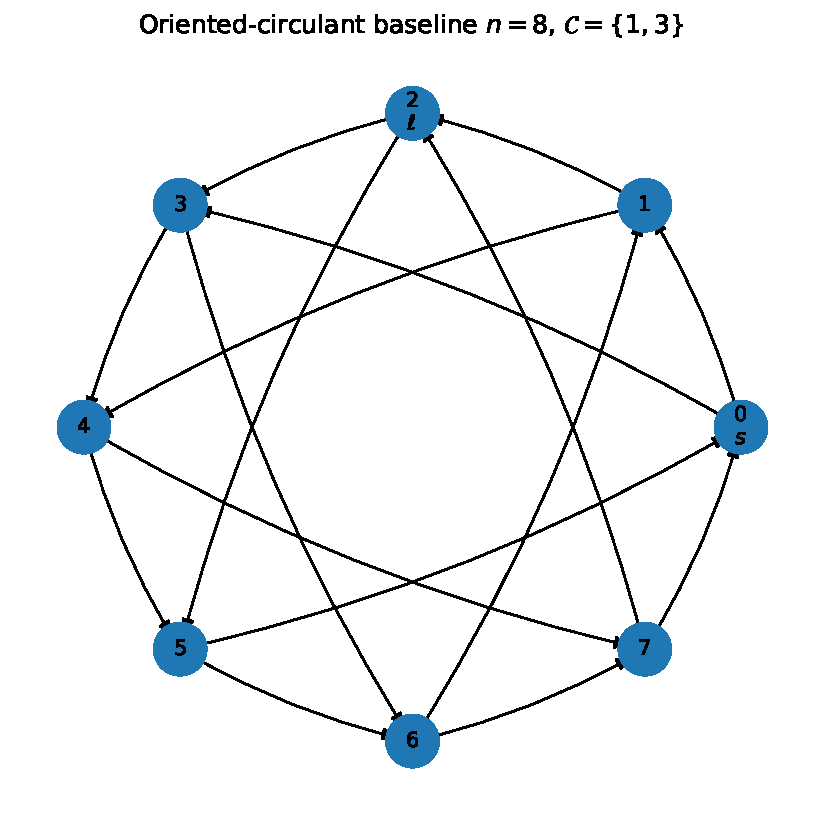
\includegraphics[width=0.58\linewidth]{figures/n8_baseline_graph.pdf}
\caption{The oriented-circulant baseline $n=8$, $\mathcal C=\{1,3\}$, with marked source $s=0$ and target $\ell=2$. The zero-transfer status of displacement $2$ is part of the public Song--Lin census.}
\label{fig:n8graph}
\end{figure}

The spectral fibres are
\begin{equation}\label{eq:n8fibres}
M_0=\{0,2,4,6\},\qquad
M_- =\{1,3\},\qquad
M_+=\{5,7\},
\end{equation}
with poles $0,-2\sqrt2,+2\sqrt2$ and weights $1/2,1/4,1/4$. Each marked sum at displacement $2$ vanishes. The common diagonal Green function is therefore
\begin{equation}\label{eq:d8}
d(z)=\frac{1}{2z}
+\frac{1}{4(z+2\sqrt2)}
+\frac{1}{4(z-2\sqrt2)}
=\frac{z^2-4}{z(z^2-8)}.
\end{equation}

Consider the affine one-event family
\begin{equation}\label{eq:affineA}
A(t)=\bigl((1-t)\ket2+(1+t)\ket0\bigr)\bra0.
\end{equation}
The amplitude pair is unimodular because $(1-t)+(1+t)=2$. Hence the rank-one coefficient and all three projected image ranks remain one for every parameter value. By \cref{prop:oneevent},
\begin{equation}\label{eq:affinegh}
g(t)=t-1,
\qquad
h(t)=t+1,
\end{equation}
up to the chosen monic normalisation. Neither factor is an architecture factor.

\begin{table}[t]
\centering
\caption{Specialisations of the affine family \eqref{eq:affineA}. All coefficient and projected-image ranks remain one.}
\label{tab:affine}
\begin{tabular}{@{}llll@{}}
\toprule
Parameter & $\Kzero$ & Nonzero declared arrows & $\Kmax$\\
\midrule
$t=1$ & all three blocks & all nine & all three blocks\\
$t=-1$ & $0$ & none & $0$\\
$t\neq\pm1$ & $0$ & all nine & $0$\\
\bottomrule
\end{tabular}
\end{table}

\begin{figure}[t]
\centering
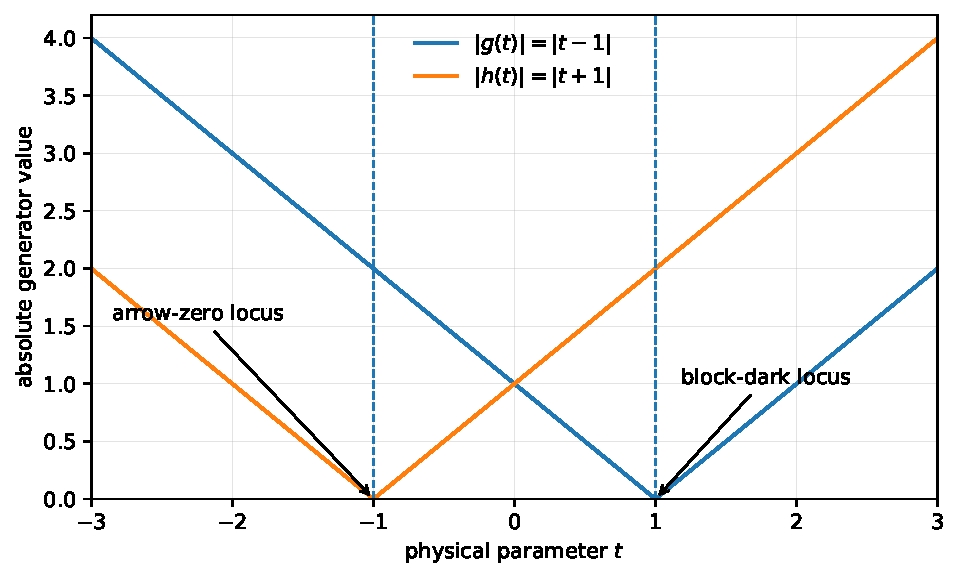
\includegraphics[width=0.72\linewidth]{figures/affine_block_edge_loci.pdf}
\caption{Illustration of the independent parameter loci in the affine family. The block generator $g=t-1$ vanishes at $t=1$, whereas the arrow generator $h=t+1$ vanishes at $t=-1$. The plot is illustrative; the loci follow exactly from \eqref{eq:affinegh}.}
\label{fig:affineloci}
\end{figure}

The physical marked resolvent gives the same separation directly:
\begin{equation}\label{eq:n8resolvent}
\bra2(zI-H_0-\eps A)^{-1}\ket0
=
\frac{\eps(1-t)d(z)^2}{1-\eps(1+t)d(z)}.
\end{equation}
At $t=1$ the entire marked transfer is zero for every $\eps$ and $z$ for which the resolvent exists. At $t=-1$ the denominator loses its return term, but the first response remains nonzero. Thus ``dark block'' and ``no declared continuation'' are genuinely different statements even in this simple family.

\section{Static arithmetic does not determine the parameter loci}\label{sec:boundary}

The preceding reduction also gives a useful boundary observation. Keep the same baseline, marked pair and declared model, but let $f(t)\in K[t]$ be arbitrary. If
\[
A_f(t)=\bigl(f(t)\ket2+\ket0\bigr)\bra0,
\]
then \cref{prop:oneevent} gives
\[
g=\operatorname{norm}(f),\qquad h=1.
\]
If instead
\[
\widetilde A_f(t)=\bigl(\ket2+f(t)\ket0\bigr)\bra0,
\]
then
\[
g=1,\qquad h=\operatorname{norm}(f).
\]
This is an immediate scaling consequence of the rank-one formula and content algebra, not a separate general impossibility theorem. Its role is conceptual: even complete static Fourier data for the baseline cannot determine the physical parameter loci when the permitted amplitude polynomial itself is allowed to vary. The baseline arithmetic certifies the dark geometry on which the perturbation acts; it does not replace the perturbation data.

\section{A bounded seven-block calculation on the eight-site baseline}\label{sec:locked}

We finally record an exact calculation for a fixed seven-block model on the same published eight-site baseline. We retain this bounded calculation in the main text because it is the paper's principal exact worked classification. We make no priority claim for its precise arithmetic pattern.

Consider
\begin{equation}\label{eq:lockedfamily}
H(\eps,t)=H_0+\eps A_1+\eps^2A_2(t),
\qquad
A_1=\ket1\bra1-\ket5\bra5,
\qquad
A_2(t)=t\ket x\bra y.
\end{equation}
On the nonzero-amplitude stratum $D(t)$ the declared endpoint/delay inventory contains seven reachable one-dimensional blocks:
\begin{center}
\begin{tabular}{@{}clcc@{}}
\toprule
Block & Meaning & Fibre & Degree\\
\midrule
0 & physical endpoint & $0$ & 1\\
1 & physical endpoint & $-$ & 1\\
2 & physical endpoint & $+$ & 1\\
3 & unresolved delay memory & auxiliary & 2\\
4 & physical endpoint & $0$ & 2\\
5 & physical endpoint & $-$ & 2\\
6 & physical endpoint & $+$ & 2\\
\bottomrule
\end{tabular}
\end{center}
At $t=0$ the $A_2$ image vanishes and the canonical physical model must be rebuilt with only the three degree-one $A_1$ endpoint blocks; the four missing ambient coordinates are therefore not interpreted as new physical dark states.

The event locations are
\[
(x,y)\in\{(1,4),(3,4),(5,4),(7,4),(6,1),(6,3),(6,5),(6,7)\},
\]
and both marked directions $0\to2$ and $2\to0$ are retained. Let $\chi_4$ denote the real primitive character modulo $4$ on odd residues,
\[
\chi_4(r)=
\begin{cases}
+1,&r\equiv1\pmod4,\\
-1,&r\equiv3\pmod4.
\end{cases}
\]
The exact calculation gives the block-$4$ table in \cref{tab:chi4}. Every other reachable block has unit generator on $D(t)$, and every declared arrow has unit generator there.

\begin{table}[t]
\centering
\caption{Exact block-$4$ outcome in the fixed seven-block family on $D(t)$. The rule is marked ket/bra class plus $\chi_4$ plus direction; it is not a $\chi_4$-only statement.}
\label{tab:chi4}
\begin{tabularx}{\linewidth}{@{}X X cc@{}}
\toprule
Symbolic event location & Condition & Forward $g_4$, $0\to2$ & Reverse $g_4$, $2\to0$\\
\midrule
$x=r$ odd, $y=4$ & $\chi_4(r)=+1$, $r=1,5$ & $1$ & $1$\\
$x=r$ odd, $y=4$ & $\chi_4(r)=-1$, $r=3,7$ & $0$ & $0$\\
$x=6$, $y=r$ odd & either value of $\chi_4(r)$ & $1$ & $0$\\
\bottomrule
\end{tabularx}
\end{table}

\begin{figure}[t]
\centering
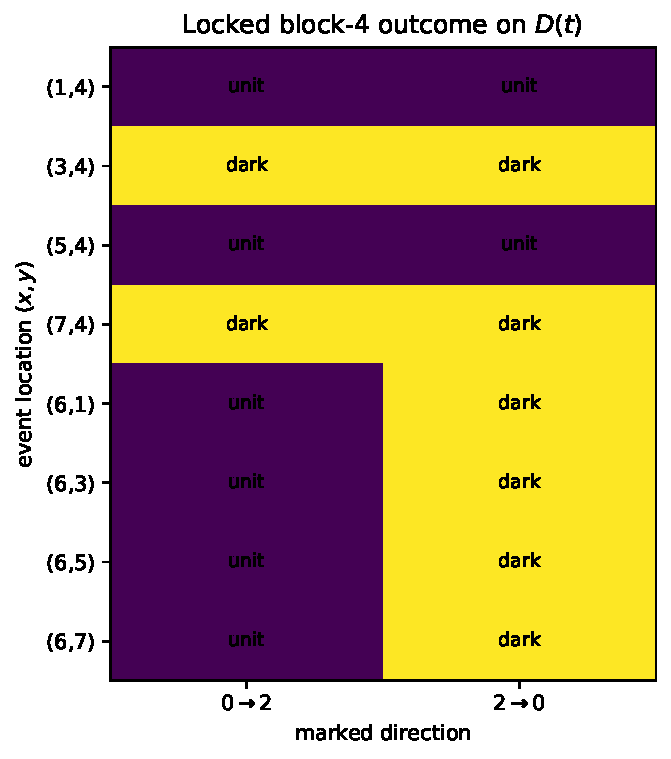
\includegraphics[width=0.58\linewidth]{figures/locked_n8_block4_map.pdf}
\caption{The sixteen marked components of the fixed seven-block calculation. ``dark'' means $g_4=0$ on $D(t)$; ``unit'' means $g_4=1$. The figure reports the bounded calculation only.}
\label{fig:lockedmap}
\end{figure}

The arithmetic behind the exceptional block is elementary once the marked fibre and orientation are fixed. For the zero fibre $M_0=\{0,2,4,6\}$,
\begin{equation}\label{eq:S0}
S_0(d)=
\begin{cases}
4,&d\equiv0\pmod4,\\
0,&\text{otherwise}.
\end{cases}
\end{equation}
For odd $r$,
\begin{equation}\label{eq:chi4sum}
S_0(1-r)=S_0(5-r)=2\bigl(1+\chi_4(r)\bigr).
\end{equation}
In the variable-ket family $(x,y)=(r,4)$, the direct block-$4$ readouts and the $A_2$ contraction vanish. The outgoing $A_1$ vector is
\begin{equation}\label{eq:ketout}
A_1G_0P_0\ket r
=\frac{1+\chi_4(r)}{4z}(\ket1-\ket5).
\end{equation}
Hence $\chi_4(r)=-1$ gives a residual-zero dead end, while for $\chi_4(r)=+1$ the first future marked readout is nonzero. In the variable-bra family $(x,y)=(6,r)$, the block-$4$ endpoint is $P_0\ket6$, independent of the odd bra site. Its forward readout is $1/(2z)$, its reverse readout is zero, and all outgoing contractions vanish. This gives the reverse-only dark cases in \cref{tab:chi4}.

Across the sixteen components the exact ledger contains 112 block generators and 204 arrow generators. Before localisation the block generators are $48$ units, $56$ copies of the architecture factor $t$, and $8$ zeros; the arrow generators are $140$ units and $64$ copies of $t$. On $D(t)$ the powers of $t$ become units, leaving $104$ unit block generators, $8$ zero block-$4$ generators, and $204$ unit arrows. In every zero case,
\[
\Kzero=\Kmax=\spanop\{e_4\};
\]
in the remaining cases both spaces vanish. The mixed response factors $2t-\ii$ and $2t+\ii$ that occur in a larger global response calculation do not occur in any block or arrow generator of this model.

\section{Discussion}\label{sec:discussion}

The calculations above separate three levels of information that are easy to conflate.

First, zero transfer is a statement about a marked scalar channel on the baseline. For circulants it is efficiently certified by spectral fibres and root-of-unity sums. Secondly, after a perturbation model is declared, a particular coordinate block is dark only when its entire finite marked future vanishes. In a one-parameter PID model this is recorded by the content generator $g_\gamma$. Thirdly, structured survival imposes an additional requirement: every declared nonzero continuation of that dark block must remain inside the dark set. This is a common invariant-kernel condition, represented in one dimension by the forward closure of the nonzero-arrow graph.

None of these distinctions requires a new general observability or invariant-subspace theorem. Their value here is organisational. The graph-theoretic arithmetic determines exact local coefficients; standard finite observability packages the complete future; coefficient content exposes the physical parameter locus; and a standard common-invariant-kernel calculation enforces the declared structure.

The affine example makes another boundary explicit. The static zero-transfer data remain fixed while the parameter roots of $g$ and $h$ can be moved by changing the physical amplitude polynomial. A classification of static spectral masks alone therefore cannot determine parameterised darkness for a family in which those amplitudes are free data. Conversely, once the amplitudes and the declared model are fixed, the content calculation is exact and finite.

There are several limitations. The perturbation in \eqref{eq:Aab} is directed and need not preserve Hermiticity or circulancy. The content-generator description is stated on one-dimensional PID strata; more general locally closed strata may require ideals rather than single polynomials. Higher-dimensional blocks replace coordinate contents by subspace/module questions. Multiple independently declared events allow more elaborate coherent cancellation, and arbitrary composite orders require a broader arithmetic analysis. These are outside the present scope.

\section{Conclusion}

Starting from known zero-transfer oriented-circulant baselines, we have organised a prescribed marked perturbation calculation around two questions: which individual declared blocks remain dark, and which of those dark blocks survive every declared continuation. Standard finite observation and coefficient content attach block and arrow parameter ideals to the model, while standard common invariant-kernel theory converts those data into structured survival. A one-event rank-one reduction shows transparently how feed-forward and return amplitudes occupy the two roles, and the published eight-site zero-transfer baseline provides a compact exact example in which their parameter loci are distinct. A separate bounded seven-block calculation illustrates how marked event type, Fourier arithmetic and direction combine in a fixed model.

The intended message is therefore not a new general observability theory. It is that zero-transfer arithmetic, parameter content and declared invariant structure can be assembled into a reproducible workflow for studying parameterised darkness on fixed graph baselines.

\appendix

\section{Strata, architecture changes and generator normalisation}\label{app:strata}

A strong architecture stratum fixes the ranks required by the declared construction, including projected coefficient-image ranks such as $\rank(P_\theta A_k)$ when those images define blocks. Exact rank conditions are locally closed, hence the coordinate ring takes the form $A_\Sigma=S^{-1}(R/I_\Sigma)$. A response zero inside such a stratum is distinct from a coefficient-rank collapse that changes the block inventory.

If $J\subseteq R$ is a block or arrow ideal, its stratum version is $JA_\Sigma$. In the one-parameter localisation $K[t,t^{-1}]$, powers of $t$ are units and are removed by normalisation. The zero ideal is represented by generator $0$; it is not assigned a monic generator. A nonzero ideal on a PID stratum is represented by a monic associate after removal of the specified stratum units.

For the locked family \eqref{eq:lockedfamily}, $t\neq0$ gives coefficient ranks
\[
\rank A_1=2,
\qquad
\rank(P_\theta A_1)=1,
\qquad
\rank A_2=1,
\qquad
\rank(P_\theta A_2)=1
\]
for each nonempty fibre. The physical endpoint/delay dimension is seven. At $t=0$, $A_2=0$ and the physical model is rebuilt with only the three degree-one $A_1$ endpoint states. Algebraically specialising a fixed seven-coordinate ambient realisation to $t=0$ is therefore not the same operation as rebuilding the physical structured model at that rank-collapse point.

\section{Content invariance under fixed coordinate changes}\label{app:content}

Let $W$ be a finite-dimensional $K$-space of proper rational functions with a fixed parameter-independent denominator. Two fixed coordinate bases of $W$ are related by some $C\in\operatorname{GL}_m(K)$. If a residual has coordinate vectors $x$ and $y=Cx$, the entries of $y$ lie in the ideal generated by the entries of $x$, while $x=C^{-1}y$ gives the reverse containment. Hence the coefficient ideal is independent of the chosen fixed rational-function basis.

Likewise, multiplication by a fixed monic polynomial $Q(z)\in K[z]$ preserves parameter content on its image: polynomial division recovers the original coefficient vector by a $K$-linear triangular map. This justifies clearing fixed baseline denominators. In contrast, clearing $1/z$ by the parameter-dependent denominator $tz$ would replace the unit content $(1)$ by the false factor $(t)$, and is therefore inadmissible.

Coherent recombination must also precede content extraction. For example,
\[
1+(t-1)=t
\]
has content $(t)$, whereas the sum of the separate ideals $(1)+(t-1)$ is the unit ideal. The shortest cancellation is $1+(-1)=0$ although both summand ideals are units. These elementary examples are why the paper keeps exact amplitudes until after declared contributions have been added.

\section{Order-nine cross-field example}\label{app:n9}

For completeness, a second certified baseline uses $n=9$ and connection set $\mathcal C=\{3\}$. The graph is the disjoint union of three directed triangles, so connectedness is not claimed. With marked sites $s=0$, $\ell=1$, the fibres are
\[
\{0,3,6\},\qquad \{1,4,7\},\qquad \{2,5,8\},
\]
at poles $0,-\sqrt3,+\sqrt3$. Each has weight $1/3$ and the source-target projector sums vanish. The diagonal Green function is
\[
d(z)=\frac{z^2-1}{z(z^2-3)}.
\]
Here the distinction between arithmetic and response fields is visible: the marked sums lie in $K_{\rm Song}=\mathbb Q(\zeta_9)$, whereas a convenient response field containing the real poles is $K=\mathbb Q(\zeta_{36})$. The same affine amplitudes $a=1-t$, $b=1+t$ give $g=t-1$ and $h=t+1$ by \cref{prop:oneevent}.

\section{Exact verification summary}\label{app:verification}

The source computation retained sixteen locked eight-site components, 112 block generators and 204 arrow generators. The paper package contains a compact data extract and an independent exact-check script. The script constructs the eight-site Hermitian adjacency, verifies
\[
H_0^3=8H_0,
\]
checks eigenvalue multiplicities $4,2,2$, verifies the $0\to2$ baseline moments through the finite horizon, reconstructs
\[
d(z)=\frac{z^2-4}{z(z^2-8)},
\]
and checks the first three event grades of \eqref{eq:scalar-oneevent} symbolically. It also verifies the locked generator counts and that precisely eight of the sixteen marked directions have dark block $4$.

The exact ledger reports early unit-content witnesses for every non-dark block: $60$ at grade $0$, $32$ at grade $1$, $8$ at grade $2$ and $4$ at grade $3$. These grades are computational certificates in the fixed presentation, not invariants under arbitrary reparametrisation of the state or grade structure. The machine calculations support the finite census; they do not substitute for the all-parameter arguments in the main text.

\section*{Transparency statement}
The mathematical organisation, manuscript drafting, and numerical diagnostic scripting in this document were developed with assistance from ChatGPT and Gemini. These tools are not authors and cannot take responsibility for correctness. The named human authors are responsible for checking the mathematics, validating computations, verifying citations, auditing generated code and data, and deciding whether the manuscript is suitable for dissemination or submission.

\section*{Data and code availability}
The accompanying reproducibility package contains the figure-generation script, a compact JSON extract of the exact census used in the tables, and an independent symbolic verification script. The larger project ledgers from which the extract was prepared are not required to compile the manuscript. No numerical tolerance is used in the exact checks; floating-point evaluation is used only to draw the illustrative generator plot.

\printbibliography

\end{document}
